\section{Automatic Feature Extraction}\label{sec:automaticExtraction}
Astronomers pay careful attention to unusual drastic behaviors of blazars, such as flare and rotation.
As a first step to identify flares and rotations (\textbf{G2}),
we have implemented automatic feature extraction for discovery and analysis of dynamic time variations (\textbf{T3}).
TimeTubesX automatically extracts three types of feature: anomalies (Section~\ref{sec:anomalyDetection}), flares (Section~\ref{sec:flareDetection}), and rotations (Section~\ref{sec:rotationDetection}).
% As the first step for quickly finding such behaviors, 
% TimeTubesX supports automatic feature extraction for three types of features: anomalies, flares, and rotations. %; flare detection; and rotation detection. 
We have significantly improved the detection algorithms for flares and rotations, compared with the ones in our paper~\cite{Sawada2018}, 
to identify flares more flexibly and detect rotations more accurately.
% The automatic feature extraction allows users to quickly identify candidate time intervals for known blazar behaviors.
%It supports the users' efficient analysis through quick access to candidates for observable behaviors.
Fig.~\ref{fig:querySpecificationPanel} (A) shows the automatic feature extraction panel, %query specification panel
where users can select the specific patterns and parameters for the automatic feature extraction.
%the users select what to detect and then input parameters for matching.
%3D tube views for the time intervals including an anomaly, flare, and rotation are provided in
The node (A) in Fig.~\ref{fig:framework} shows example TimeTubes views for an anomaly, flare, and rotation.
% all three supported blazar patterns (i.e., anomaly, flare, rotation).

\subsection{Anomaly Detection}\label{sec:anomalyDetection}
It is challenging for astronomers to manually identify time variations across multiple variables. 
We define time points with drastic temporal changes over polarization, intensity, and color as \textit{anomalies}.
Tracking anomalies can result in identifying unusual time variations or presages of well-known behaviors such as flares or rotations
because observable blazar behaviors show a tendency to include these drastic variations.

The anomaly degree was defined in our previous paper~\cite{Sawada2018} as the product of the change amount over polarization, intensity, and color per day:
\begin{equation*}
\begin{split}
  \int_t^{t + \Delta t}\left|\frac{dPolar(t)}{dt}\right|\cdot\left|\frac{dI(t)}{dt}\right|\cdot\left|\frac{dC(t)}{dt}\right|dt,
  \label{eq:anomaly}
\end{split}
\end{equation*}
where $Polar(t)$ means the position of a data sample on the Stokes plane at time $t$, and $I(t)$ and $C(t)$ stand for intensity and color, respectively. 
%In the anomaly detection, observation errors have not been taken into account for the sake of simplicity.

\textsf{Experimental results.\ } When we applied the anomaly detection to our synthetic data, 
data samples around an extreme peak (orange diamonds in Fig.~\ref{fig:synthesisData}~(a)) and parts of dynamic rotations (green plots in (b)) were highly ranked.


%
%
\subsection{Flare Detection}\label{sec:flareDetection}
Flares are defined as extreme peaks of brightness (i.e., emitted light intensity). 
Astronomers regard flares as one of the most important observed behaviors of blazars.
However, since there is no specific threshold value of $I$ to define a flare, 
they need to analyze the local temporal profile of $I$ to identify flares.
We have updated flare detection methods from those in our previous paper~\cite{Sawada2018}
to detect relatively small local flares as well as globally large flares.
To that end, we utilize peak detection methods for time-series data~\cite{Palshikar2009} to extract flare candidates. 
The flare detection comprises the following two steps:
\begin{enumerate}[nosep, label=\textsl{Step \arabic*}, align=parleft, leftmargin=*]
    \item \textsl{Compute the spikiness score $S$ for each of data samples}; \label{algo:flareSpikiness}
    \item \textsl{Filter out data samples with globally small $S$}. \label{algo:flareFilter}
    % whose $S$ is small in a global context}. \label{algo:flareFilter}
\end{enumerate}
TimeTubesX uses Equation~\ref{equ:S2} to compute the spikiness score $S$ for \ref{algo:flareSpikiness},
because we tested multiple equations for $S$ and empirically found that the following produces the best results.
\begin{eqnarray}
    % S_1 &=& \frac{\underset{1 \leq k \leq K}{\max}\{x_i - x_{i - k}\} + \underset{1 \leq k \leq K}{\max}\{x_i - x_{i + k}\}}{2}\label{equ:S1}\\
    S &=& \frac{\frac{\sum_{k=1}^{K}(x_i - x_{i - k})}{K} + \frac{\sum_{k=1}^{K}(x_i - x_{i + k})}{K}}{2}\label{equ:S2},
    % S_3 &=& \frac{\left(x_i - \frac{\sum_{k=1}^{K}{x_{i - k}}}{K}\right) + \left(x_i - \frac{\sum_{k=1}^{K}{x_{i + k}}}{K}\right)}{2}\label{equ:S3}
\end{eqnarray}
where $x_i$ denotes a data sample indexed as $i$ and $K$ denotes the number of neighbors that should be examined.
% \autoref{equ:S1} computes the average of the maximum differences between a focused data sample $x_i$ and $K$ left and right neighbors of $x_i$.
Equation~\ref{equ:S2} provides the average value of the averages of distances between $x_i$ and $K$ left neighbors and those between $x_i$ and $K$ right neighbors.
% \autoref{equ:S3} computes the average of distances between $x_i$ and the mean of $K$ left and right neighbors. 
% Because flares tend to have small peaks before or after the flare, 
\ref{algo:flareFilter} retains only data samples that satisfy $S - \bar{S} > h \times \sigma_{S}$, 
where $\bar{S}$ and $\sigma_{S}$ denote the mean and standard deviation of all computed $S$ for the dataset, respectively, 
and $h$ is a user-specified sensitivity threshold. 
The original algorithm~\cite{Palshikar2009} merges peaks that are close together into one, 
but we did not adopt this strategy
because astronomers are equally interested in both small, individual flares and large, aggregated flares.
% also interested in small individual flares rather than just big aggregated flares.

\begin{figure}[tb]
    \centering
    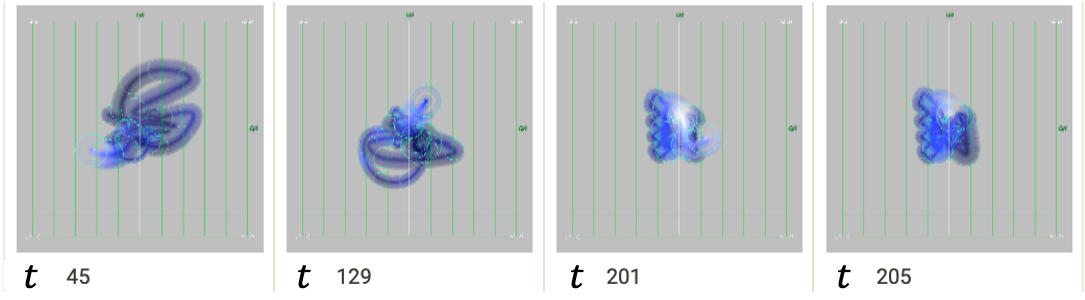
\includegraphics[width=.85\linewidth]{vgtc_journal_latex/figures/flareDetectiondemodataResults.png}
    \caption{Flare detection results for our synthetic data. The detected results match the four red data points in Fig.~\ref{fig:synthesisData}~(a).}
    \label{fig:flareDetection}
\end{figure}
\begin{figure}[tb]
    \centering
    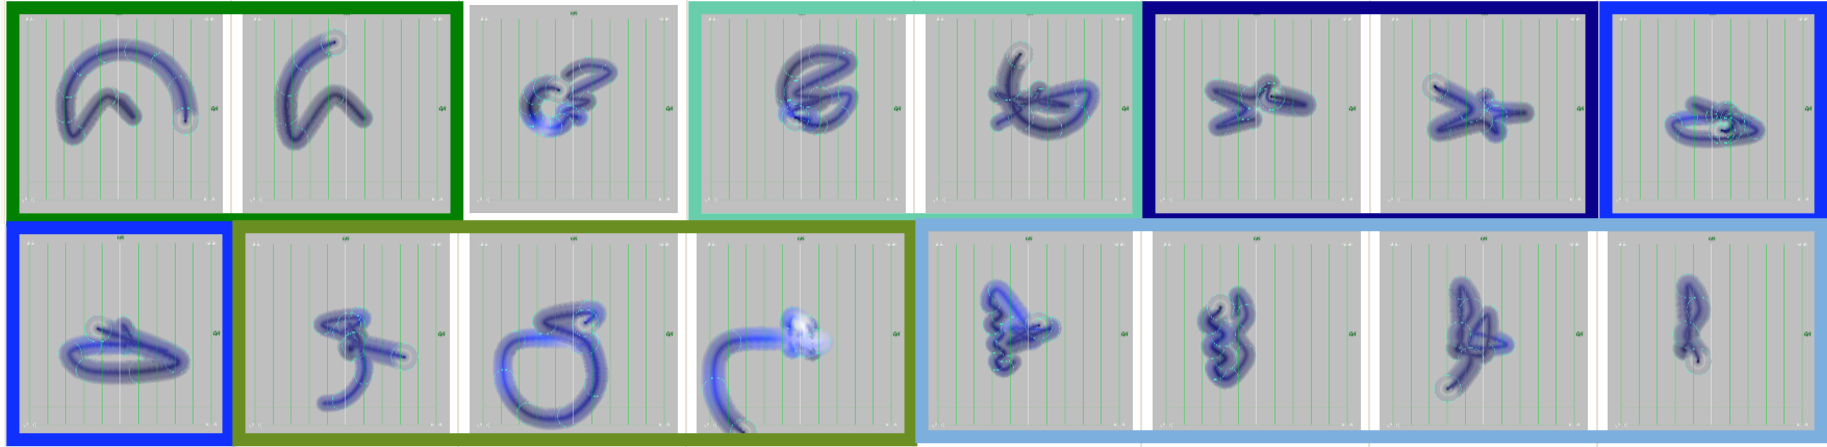
\includegraphics[width=\linewidth]{vgtc_journal_latex/figures/rotationDetectiondemodataResultsOR.png}\\
    \footnotesize{\sf(a) Previous rotation detection method~\cite{Fujishiro2018}.}\\
    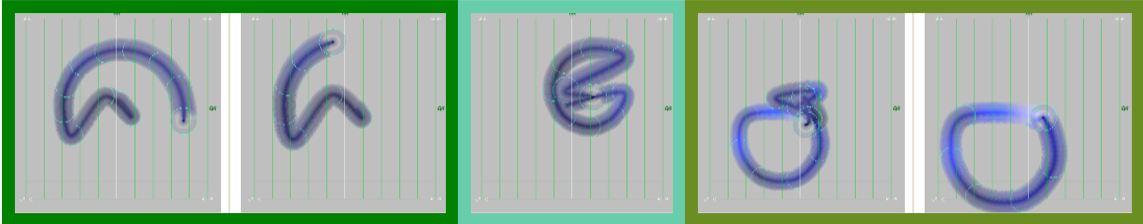
\includegraphics[width=.8\linewidth]{vgtc_journal_latex/figures/rotationDetectiondemodataResults.png}\\
    \footnotesize{\sf(b) Our improved method.}
    \caption{Rotation detection results for our synthetic dataset in Fig.~\ref{fig:synthesisData}. 
        The outline color corresponds to the color in Fig.~\ref{fig:synthesisData}~(b).
        Our previous method detects narrow patterns and noise (blue), 
        whereas our improved method detects only big rotations (green).}
    \label{fig:rotationResults}
\end{figure}
\textsf{Experimental results.\ } We applied the flare detection to our synthetic data.
We set $K$ and $h$ to 3 and 1, respectively.
Fig.~\ref{fig:flareDetection} presents the flare detection results.
The four time points were detected as flares,
which completely coincide with the deliberately generated peaks that are highlighted in orange in Fig.~\ref{fig:synthesisData}~(a).

\subsection{Rotation Detection}\label{sec:rotationDetection}
The polarization rotation is another important observed behavior of blazars. 
Astronomers do not yet agree on whether rotation is a real feature or just a result of random variations of polarization.
To validate their hypotheses, they scrutinize correlations between polarization and other properties of the time interval.
They have been analyzing time variation of $PA$ to identify rotations~\cite{Ikejiri2011, Uemura2017},
but the rotation center will not be located at the origin of the Stokes plane ($(q, u) = (0, 0)$) when there are multiple polarized components in the sky.
Thus, estimating a rotation only by $PA$ may not allow astronomers to adequately understand its behavior.
Our rotation detection is capable of addressing any rotations regardless of the position of the rotation center.

We use a sliding window approach that allows users to manually define the length of the time interval for the sliding window. Based on reports by astronomers~\cite{Sasada2012}, we set the default window size to between three and four weeks.
%Using a sliding window approach, the rotation detection picks up a time interval from a long-term dataset. 
%Users can freely determine the time interval length, 
%whose default setting we empirically decided from three weeks to a month according to the prior report by the astronomers~\cite{Sasada2012}.

Computation of the rotation angle is divided into the following seven steps:
\begin{enumerate}[nosep, label=\textsl{Step \arabic*}, align=parleft, leftmargin=*]
    \item \textsl{Compute weighted means ($\overline{q}, \overline{u}$) of $q$ and $u$ of the time interval};\label{algo:rotationMean}
    \item \textsl{Compute standard deviations ($\sigma_{q}, \sigma_{u}$) of $q$ and $u$ of the time interval}; \label{algo:rotationStd}
    \item \textsl{Convert the rectangular coordinates ($q-u$ domain) to the polar coordinates ($r - \theta$ domain) with its origin shifted to $(\overline{q}, \overline{u})$}; \label{algo:rotationPolar}
    \item \textsl{Filter out time intervals whose $\sigma_{q}$ or $\sigma_{u}$ are smaller than standard deviations of the entire dataset}; \label{algo:rotationFilter}
    \item \textsl{Compute the difference ($\theta_{\rm diff}$) of $\theta$'s of two consecutive data samples}; \label{algo:rotationDiff}
    \item \textsl{Sum up $\theta_{\rm diff}$'s to yield $\theta_{\rm sum}$}; \label{algo:rotationSum}
    \item \textsl{Check whether $\theta_{\rm sum}$ is larger than the user-specified threshold for the total rotation angle}. \label{algo:rotationThreshold}
\end{enumerate}
To avoid misleading effects of outliers and unexpected values at the edges of a time interval,
our detection method uses weighted mean values at \ref{algo:rotationMean}. Smaller weights are assigned to both ends of the time interval, 
while heavier weights are assigned to its center according to a Gaussian distribution. %as the rotation center of the focused time interval at \ref{algo:rotationMean}.
Note that users are allowed to adjust these weight ratios.
%
To avoid misclassifying time intervals with large $q$ or $u$ variance and unlike rotations as rotation candidates,
we have improved upon our previous rotation detection method~\cite{Sawada2018} based on feedback from two astronomers at Hiroshima University~\cite{Huang2019}.
%
%In our previous short paper~\cite{Sawada2018}, 
%we filter out only time intervals \textbf{both} of whose $\sigma_{q}$ \textbf{and} $\sigma_{u}$ are smaller than the standard deviation of the entire dataset. 
%However, several astronomers in Hiroshima University reported that the previous rotation detection sometimes detects time intervals with large $q$ or $u$ variance and unlike rotations~\cite{Huang2019}.
%To address this problem, the current 
%
To detect only large rotations, 
our new rotation detection method is able to filter out time intervals in which \textbf{either} $\sigma_{q}$ \textbf{or} $ \sigma_{u}$ is smaller than the standard deviation of the entire dataset. % avoid small or narrow patterns.
%The up-to-date version provides 
Note that this and other provided filtering constraints also allow for discovery of small or narrow rotations, such as red and blue patterns in Fig.~\ref{fig:synthesisData}~(b).
% Additionally, we provide multiple filters on standard deviations of the time intervals as well as the previous filter, to find out small rotations.
%
At \ref{algo:rotationDiff}, we cannot compute $\theta_{\rm diff}$ simply by subtracting $\theta$'s of consecutive observations 
due to the range constraint on $\theta_{\rm diff}$, i.e., $\theta_{\rm diff} \in [0, 2\pi]$. 
For example, when two successive data samples are located in the first and fourth quadrant of the Stokes plane, 
we need to consider whether to take the clockwise or counterclockwise direction as $\theta_{\rm diff}$. 
So, we determine the rotation direction 
by checking increasing/decreasing tendency in $\theta$'s with exponential smoothing~\cite{Brown1956}.
% by comparing the predictive values for $\theta$'s, which we can derive by exponential smoothing~\cite{Brown1956}.
% which is a forecasting method
% for time-series datasets to predict a subsequent value based on previous values. 
% that produces a weighted average of past observations. 
It forecasts the next value according to past observations by assigning larger weights to more recent observations.
It will address the uncertainty about the rotation direction and make results more feasible (\textbf{T1}).
% If the predictive value derived by exponential smoothing increases, 
% the rotation direction tends to be counterclockwise;
% otherwise, it is clockwise.
We estimate the variation trend of $\theta$ and
then choose the angle in the predicted rotation direction as $\theta_{\rm diff}$.
Users can set an arbitrary angle as a threshold parameter at \ref{algo:rotationThreshold}.

\textsf{Experimental results.\ } To compare our novel algorithm with the previous rotation detection algorithm~\cite{Sawada2018}, we applied both to our synthetic dataset.
As the results in Fig.~\ref{fig:rotationResults}~(a) show, 
the previous algorithm detects not only big rotations (green patterns in Fig.~\ref{fig:synthesisData}~(b)) but also narrow or rough-edged patterns (blue).
The improved algorithm is more accurate and detects only time intervals in which the polarization values dynamically rotate (green), as shown in Fig.~\ref{fig:rotationResults}~(b).
% Note that users can also detect small or narrow rotations such as red or blue patterns in \autoref{fig:synthesisData}~(b) 
% by changing filtering constraints on $\sigma_{q}$ and/or $ \sigma_{u}$.
% The previous method detects time intervals which have large variances in the $x$ or $y$ axis direction as rotation candidates. 
% Some of them seem to just behave messily and not rotate. 
% We apply the improved method to the same synthetic data. 
% The detection results are displayed in Fig.~\ref{fig:rotationResults}~(b). 
% In comparison with (a), it seems that time intervals with messy variations are omitted from the results. 
% With the improvements, the up-to-date rotation detection can find out time intervals where the polarization values dynamically rotate.

% \subsection{Anomaly and flare with a rotation}
% Some astronomers reported that rotations tend to co-occur with flares~\cite{Ikejiri2011}.
% The automatic feature extraction can find out a rotation including anomalies or flares inside its time interval 
% by combining the anomaly detection in \autoref{sec:anomalyDetection} or the flare detection in \autoref{sec:flareDetection} with rotation detection in \autoref{sec:rotationDetection}.



% We improve the detection algorithms for the initial version of the automatic feature extraction in \cite{Sawada2018}. 

% The following parts dig into each of the options.
% The automatic feature extraction is particularly important for task \textbf{T3}.


% TODO: Update figures!
% \begin{figure}[tb]
%     \centering
%     \begin{minipage}{.44\linewidth}
%         \centering
%         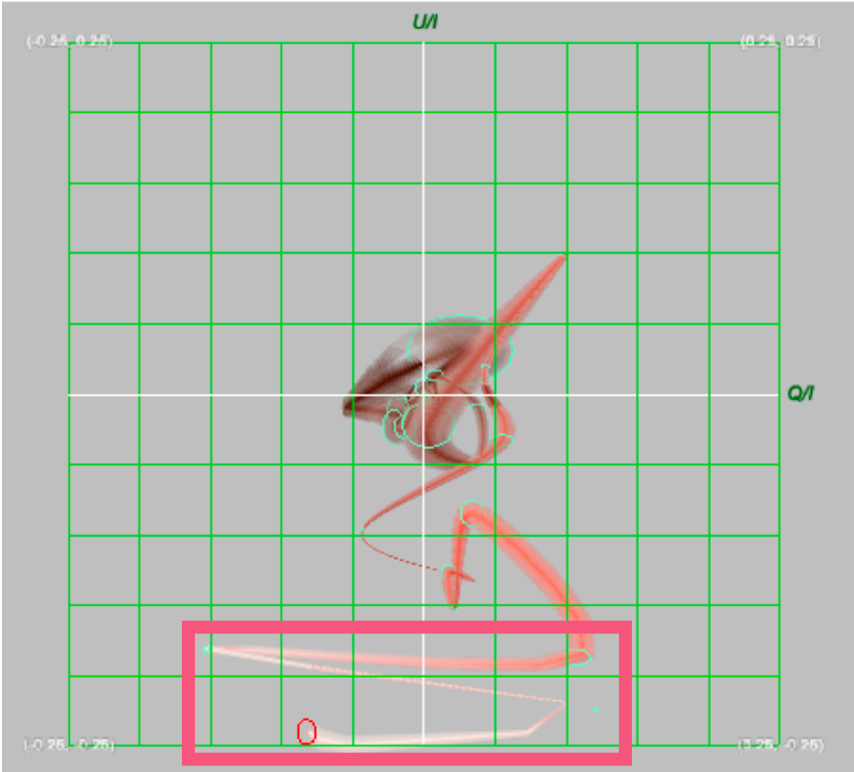
\includegraphics[width=0.99\linewidth]{vgtc_journal_latex/figures/flareExampleTimeTubes.png}
%     \end{minipage}
%     \begin{minipage}{.55\linewidth}
%         \centering
%         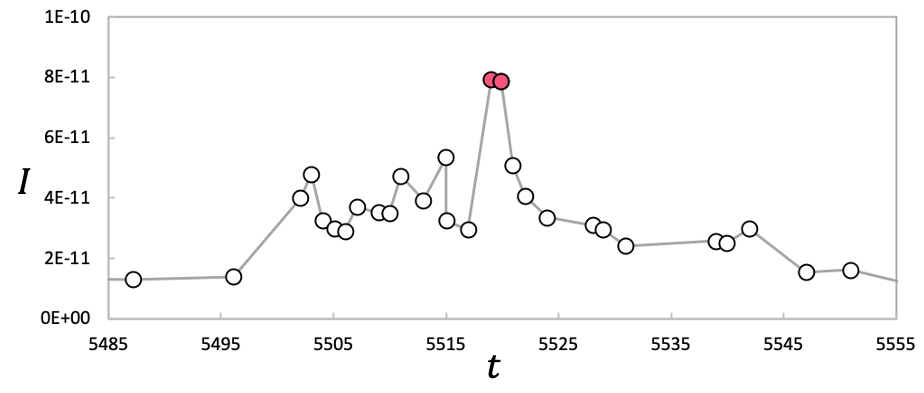
\includegraphics[width=.99\linewidth]{vgtc_journal_latex/figures/flareExampleSP.png}
%     \end{minipage}
%     \begin{minipage}{.44\linewidth}
%         \centering
%         \textsf{\footnotesize (a)~TimeTubes view.}
%     \end{minipage}
%     \begin{minipage}{.55\linewidth}
%         \centering
%         \textsf{\footnotesize (b)~Light curve.}
%     \end{minipage}
%     \caption{Flare of a blazar \textbf{3C 454.3} at $t=5{,}518.98$. The flare part is highlight in red in both of TimeTubes and scatterplots views.}
%     \label{fig:flareExample}
% \end{figure}

% In \autoref{fig:flareExample}, 
% a flare occurrence in the blazar, named \textbf{3C 454.3}, around $t = 5{,}518.98$ is visualized by TimeTubes~(a) and light curve~(b).
% In such a short period, the intensity drastically increases and decreases. 
% In (a), the color of the tube looks much brighter in the part enclosed by a red rectangle than the other parts.
% Data samples enclosed by the red rectangle in (a) coincide with red plots in (b).

% though the time intervals with sharp peaks are considered to be flares.

% To test the flare detection, we used a synthetic data in \autoref{fig:synthesisData}.
% In (a), a square plot means the first data sample, while a triangular the last data sample.


% \begin{figure}
%     \begin{minipage}{0.49\linewidth}
%         \centering
%         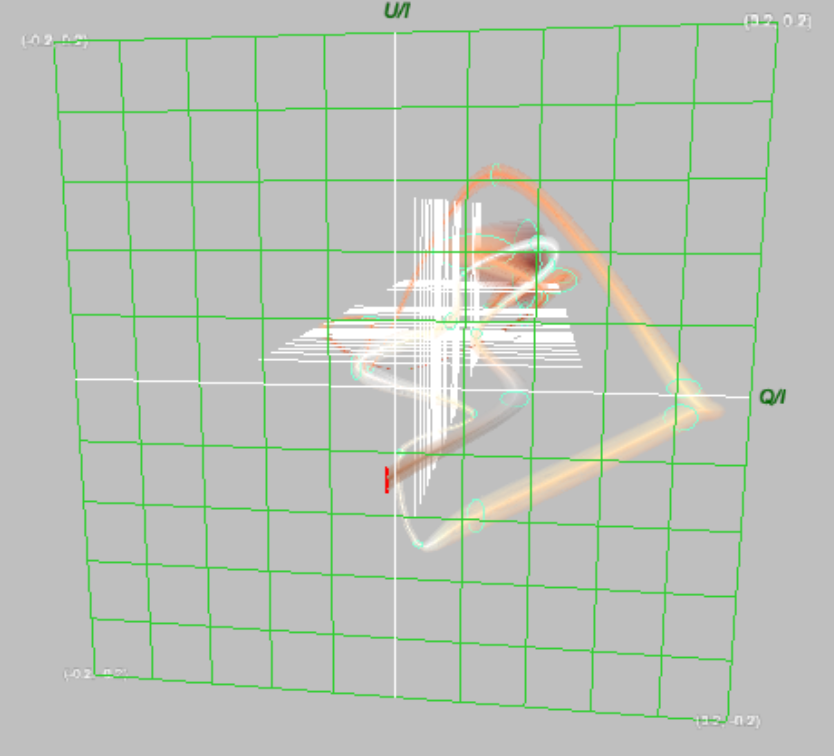
\includegraphics[width=.95\linewidth]{vgtc_journal_latex/figures/TimeTubes_rotation.png}
%         \footnotesize{\sf (a)~TimeTubes view.}
%     \end{minipage}
%     \begin{minipage}{0.49\linewidth}
%         \centering
%         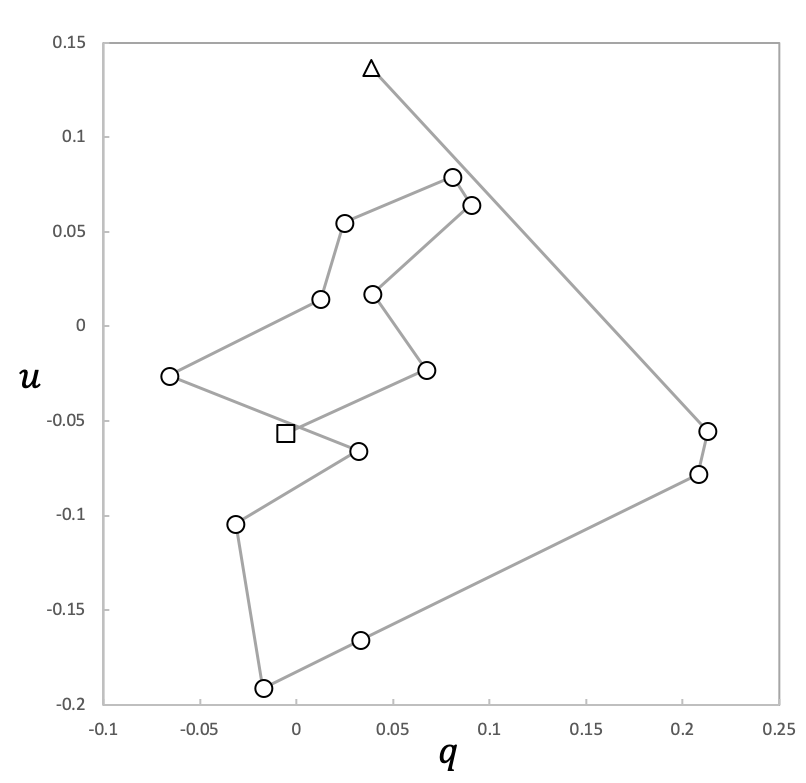
\includegraphics[width=.95\linewidth]{vgtc_journal_latex/figures/ScatterPlot_rotation.png}
%         \footnotesize{\sf (b)~Scatterplots view.}
%     \end{minipage}
%     \caption{Rotation of \textbf{3C 454.3} in the time interval $[5{,}156, 5{,}186]$. TimeTubes view provides an oblique view to show 3D structure of the tube. We connect data samples in chronological order, where the period starts from a square plot and end at a triangular plot.}
%     \label{fig:rotationExample}
% \end{figure}

% The dynamic rotation on the Stokes plane can be characterized with variation of $PA$ in \autoref{eqn:PA}.

% It is still controversial among the astronomers. 

% \autoref{fig:rotationExample} shows TimeTubes view~(a) and scatterplots view~(b) of the time interval $[5{,}156, 5{,}186]$ for \textbf{3C 454.3} including a behavior regarded as a rotation. 
% \autoref{fig:rotationExample}~(b) shows scatterplots for the Stokes plane,
% where the plots are connected with a polygonal line in chronological order,
% where the rotating behavior starts from a square plot and ends at a triangular plot.
% The polarization values do not necessarily rotate around the origin of the Stokes plane, 
% that is $(q, u) = (0, 0)$, as shown in \autoref{fig:rotationExample}.
% due to the inconsistent position of the rotation center.


% We recommend users to use the weighted mean instead of the arithmetic mean 
% because outliers or unexpected values at the edges of the time interval can directly affect the arithmetic mean.


% whereas the previous version filters out only time intervals \textit{both} of whose standard deviations of $\sigma_{Q/I}$ and $ \sigma_{U/I}$ larger than them. %the global standard deviations.
% With this improvements, the up-to-date version detects only time intervals where the polarization values dynamically rotate.

% \begin{figure}[tb]
%     \centering
%     \includegraphics[width=.99\linewidth]{images/RotationDetectionOR.png}\\
%     \footnotesize{\sf (a)~Previous method.}\\
%     \includegraphics[width=.99\linewidth]{images/RotationDetectionAND.png}\\
%     \footnotesize{\sf (b)~Improved method.}
%     \caption{The rotation detection results for a randomly generated synthetic data. 
%         (a)~Time intervals with large variance are also detected as rotations.
%         (b)~Time intervals which vary largely in both of $x$ and $y$ axes directions are detected.
%     }
%     \label{fig:rotationResults}
% \end{figure}